\chapter{Grundlagen}
\label{grundlagen}
In diesem Kapitel werden die benötigten Grundlagen erläutert, um ein besseres Verständ\-nis für die Optimierungen der einzelnen Architekturen und das weitere Vorgehen mittels Quantisierung und Pruning zu erhalten.
Dazu werden zuerst die wichtigsten Grundlagen zu Feedforward-Netzen und Convolutional Neural Networks besprochen. Im Anschluss daran werden aufbauend auf diesen Grundlagen optimierte Schichten erläutert, welche dann in dem folgenden Abschnitt über Architekturen für mobile und eingebettete Systeme Anwendung finden. Nach dem Abschnitt über die Architekturen folgen noch in zwei Abschnitten die Grundlagen zu Quantisierung und Pruning. 



\section{Künstliche neuronale Netze}
Bei künstlichen neuronalen Netzen handelt es sich um ein Modell der Informatik, welches angelehnt an ein biologisches Gehirn ist. Künstliche neuronale Netze, kurz KNNs, sind in der Lage durch einen Trainingsprozess mathematische Funktionen zu approximieren. Aus diesem Grund finden die KNNs häufig dort Anwendung, wo es einfacher ist ein lernfähiges KNN zu trainieren als für das gegebene Problem einen Algorithmus oder eine Funktion zu entwickeln, die das Problem direkt löst. Es gibt eine Vielzahl verschiedener Arten von künstlichen neuronalen Netzen. Zwei populäre und auch für diese Arbeit relevanten Arten sind die Feedforward-Netze und die Convolutional Neural Networks.
Die Erläuterungen in diesem Abschnitt sind angelehnt an das Grundlagenwerk von Jörg Frochte \cite{frochte_maschinelles_2019}.


\subsection{Feedforward-Netze}
\label{FFNN}
Bei Feedforward-Netzen handelt es sich um ein Modell, welches in Schichten organisiert ist (Einschichtige/Mehrschichtige Feedforward-Netze). Jede Schicht besteht aus einem oder mehreren Neuronen. In der Regel, aber nicht notwendigerweise, ist jedes Neuron der vorhergehenden Schicht mit jedem Neuron der nachfolgenden Schicht verbunden. Ein Neuron ist lediglich ein Knoten in dem resultierenden Graphen. An den Kanten des Graphen sind Gewichte, welche die Parameter sind, die ein Feedforward-Netz lernt.

\begin{figure}[htbp]
\centerline{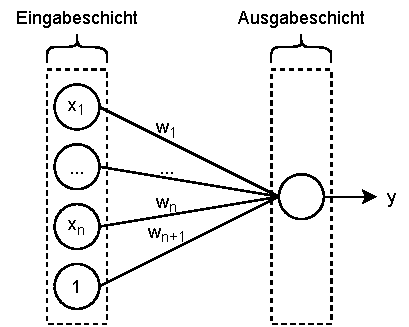
\includegraphics[width=0.5\textwidth]{content/images/FFNN.pdf}}
\caption{Einschichtiges Feedforward-Netz Eingabeschicht, Bias und einer Ausgabeschicht mit einem Neuron}
\label{f2.1}
\end{figure}

In Abbildung \ref{f2.1} ist das ein einfaches einschichtiges Feedforward-Netz mit einer Eingabeschicht und einer Ausgabeschicht mit einem Neuron dargestellt. Dieses Netz nimmt als Eingabe einen Featurevektor $\vec{x} = \left(\begin{array}{ccc} x_1 & \cdots & x_n \end{array} \right)^T$ und berechnet in diesem Fall als Ausgabe eine einzelne Zahl $y$. $y$ berechnet sich wie folgt:

\begin{equation}
y = \sigma \left( \left( \sum_{i=1}^{n} w_i \cdot x_i \right) + w_{n+1} \cdot 1 \right)
\label{eq2.1}
\end{equation} 

Als Erstes werden alle Werte der vorherigen Schicht, die mit dem Neuron in der aktuellen Schicht verbunden sind, mit den Gewichten an den jeweiligen Kanten gewichtet und aufsummiert. Dazu wird der sogenannte Bias addiert, welcher immer einen konstanten Wert besitzt (in dem Fall den Wert 1) und ebenfalls gewichtet mit dem Neuron in der Ausgabeschicht verbunden ist. Anschließend wird auf die gesamte Summe eine Aktivierungsfunktion $\sigma$ angewendet.

Bei mehr als nur einem Neuron in der Ausgabeschicht wird für jedes weitere Neuron analog vorgegangen und man erhält statt einer einzelnen Zahl einen Vektor als Ausgabe dieser Schicht. Handelt es sich um ein mehrschichtiges Feedforward-Netz, wird für jede Zwischenschicht bis zur Ausgabeschicht sukzessive diese beschriebene Technik angewendet, um den Ausgabevektor des Netzes zu erhalten.

Der Lernprozess eines solchen Feedforward-Netzes besteht darin mittels geeigneter Techniken die Gewichte anzupassen und dadurch den Fehler, den das Netz macht, zu minimieren, sodass die Ausgabe des Netzes die gewünschte Ausgabe approximiert.


\subsection{Convolutional Neural Networks}
\label{cnns}
Eine andere Art von Feedforward-Netzen sind die so genannten Convolutional Neural Networks, kurz CNNs. Diese Netze nutzen das mathematische Prinzip der Faltung (engl. Convolution), welches sich sowohl auf zweidimensionalen Daten wie Bildern, als auch auf eindimensionale Daten wie Zeitreihen anwenden lässt. Für diese Arbeit werden CNNs aber lediglich auf Bilddaten, also zweidimensionalen Daten betrachtet.

Convolutional Neural Networks werden, wie die zuvor beschriebenen Feedforward-Netze, erneut in Schichten angeordnet, jedoch werden bei den CNNs Convolutional Layer verwendet.

\begin{figure}[htbp]
\centerline{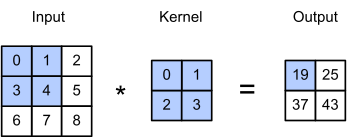
\includegraphics[width=0.5\textwidth]{content/images/convolution.png}}
\caption{Zweidimensionale Cross-Correlation auf einer Eingabe der Größe $3 \times 3$ mit einem Kernel der Größe $2 \times 2$. \cite{zhang_dive_2020}}
\label{f2.2}
\end{figure}

Ein Convolutional Layer ist eine Schicht, bei der ein Filter (Kernel) über die Eingabedaten (Input) geschoben wird. Dies wird auch Cross-Correlation oder Faltung (Convolution) genannt. Ein Beispiel für diese Cross-Correlation ist in Abbildung \ref{f2.2} dargestellt. Dabei wird der Kernel über den Eingabedaten platziert, die Werte des Kernels mit den darunterliegenden Werten der Eingabedaten multipliziert und alle Werte aufaddiert. Zusätzlich kann dann noch auf diese Summe eine Aktivierungsfunktion $\sigma$ angewendet werden. Anschließend wird der Kernel auf den Eingabedaten um eine festgelegte Schrittweite (strides) verschoben und die Prozedur wiederholt, bis der Kernel einmal über die gesamten Daten gelaufen ist. Das Ergebnis einer solchen Convolution wird auch Feature Map genannt.

Für einen Input $I$ und einen Kernel $K$ der Größe $M \times N$ kann das Ergebnis $S$ einer Cross-Correlation wie folgt formalisiert werden \cite{frochte_maschinelles_2019}:

\begin{equation}
S[i, j] = \sum_{m=1}^{M} \sum_{n=1}^{N} I[i+m, j+n] \cdot K[m, n]
\label{eq2.2}
\end{equation}

Die eckigen Klammern entsprechen in dieser Formel Zugriffe auf Elemente von Matrizen. Beispielsweise ist mit $S[i, j]$ der Wert der Feature Map in der $i$-ten Zeile und $j$-ten Spalte gemeint.

Besitzt der Input $I$ $C$ Channel (z.B. bei einem RGB-Bild $C = 3$), dann hat der Kernel $K$ die Größe $M \times N \times C$ und die Formel \ref{eq2.2} erweitert sich wie folgt:

\begin{equation}
S[i, j] = \sum_{c=1}^{C} \sum_{m=1}^{M} \sum_{n=1}^{N} I[i+m, j+n, c] \cdot K[m, n, c]
\label{eq2.3}
\end{equation}

Wird die Cross-Correlation, wie oben beschrieben, angewendet, ist die resultierende Feature Map kleiner als der Input, da der Kernel nicht über die Ränder hinauslaufen kann. Falls die Feature Map dieselbe Größe wie die Eingabe haben soll, kann ein Padding verwendet werden. Beim Padding werden die Eingabedaten an den Rändern mit Werten aufgefüllt. Eine Art des Paddings ist beispielsweise das Zero Padding, bei dem die Ränder der Eingabedaten mit Nullen aufgefüllt werden.



\section{Optimierte Schichten}
Neben den einfachen Schichten aus Neuronen oder den Convolutional Layern gibt es noch optimierte Schichten oder Kombinationen verschiedener Schichten, die eine Optimierung des Netzwerkes, in denen sie eingesetzt werden, erzielen sollen. 
Eine Auswahl solcher Optimierungen werden im folgenden vorgestellt und anschließend in Abschnitt \ref{architekturen} angewendet.


\subsection{Depthwise Separable Convolutions}
\label{depthwise_separable_convolutions}
In Abschnitt \ref{cnns} wurden die Convolutional Neural Networks mit den Convolutional Layern vorgestellt. Eine Depthwise Separable Convolution ist eine optimierte Variante der Standard-Convolution.

In der Formel \ref{eq2.3} ist dargestellt, wie eine Standard-Convolution auf Eingabedaten mit mehreren Channel arbeitet. Der Kernel der Größe $M \times N \times C$ führt auf jedem Channel eine Convolution durch und summiert im gleichen Schritt die Werte für jeden Channel zu einem Wert in der Feature Map. Bei der Depthwise Separable Convolution wurde diese Standard-Convolution aufgeteilt in die Depthwise Convolution und die Pointwise Convolution \cite{howard_mobilenets_2017}.

Die Depthwise Convolution führt auf Eingabedaten der Größe $H \times W \times C$ mit dem Kernel der Größe $M \times N \times C$ eine Convolution durch. Der Unterschied zur normalen Convolution besteht darin, dass die Ergebnisse der einzelnen Channel nicht aufsummiert werden. Dadurch bleiben die Channel in einer Depthwise Convolution erhalten. Diese Operation kann wie folgt formalisiert werden \cite{howard_mobilenets_2017}:

\begin{equation}
S[i, j, c] = \sum_{m=1}^{M} \sum_{n=1}^{N} I[i+m, j+n, c] \cdot K[m, n, c]
\label{eq2.4}
\end{equation}

Die Variable $c$ entspricht dabei dem Index eines Channel mit $1 \leq c \leq C$.

Nach dieser Depthwise Convolution Schicht folgt eine Pointwise Convolution Schicht, welche im Grunde eine normale Convolution mit einem Kernel der Größe $1 \times 1 \times C$ darstellt. Dieser Kernel bildet Linearkombinationen der einzelnen Channel und kombiniert somit die Channel zu einem einzelnen Channel. Die Menge an Channel der Feature Map einer Depthwise Separable Convolution Schicht wird durch die Anzahl der Kernel in der Pointwise Convolution Schicht gesteuert.

Durch das Aufspalten der Convolution in eine Depthwise Convolution und eine Pointwise Convolution erreicht die Depthwise Separable Convolution niedrigere Berechnungskosten und benötigt weniger Parameter \cite{howard_mobilenets_2017}. Der Faktor, um den die Berechnungskosten bei einer Depthwise Separable Convolution im Vergleich zu einer Standard-Convolution reduziert wird, beträgt \cite{howard_mobilenets_2017}:

\begin{equation}
\frac{1}{C_{out}} + \frac{1}{D_K^2}
\label{eq2.5}
\end{equation}

In Formel \ref{eq2.5} wird angenommen, dass der Kernel der Depthwise Convolution quadratisch mit der Höhe/Breite $D_K$ ist. $C_{out}$ entspricht der Anzahl an Channel in der Ausgabe der Depthwise Separable Convolution, welche sich durch die Anzahl an Kernel (Filter) der Pointwise Convolution Schicht ergibt.


\subsection{Linear Bottlenecks}
\label{linear_bottlenecks}
Eine Linear Bottleneck Schicht ist eine Kombination aus verschiedenen Convolutional Layern. Die Idee, welche hinter dieser Schicht steht, ist, dass angenommen wird, dass eine Menge von realen Bildern immer in eine niedrig-dimensionale Repräsentation eingebettet werden kann \cite{sandler_mobilenetv2_2019}. Also mit anderen Worten, die Menge an Bilder in eine komprimierte Darstellung überführt werden kann, bei denen die einzelnen Features einen höheren Informationsgehalt besitzen. Dies machen sich Linear Bottlenecks zunutze. 

Das grundlegende Prinzip hinter diesen Bottleneck Schichten ist, dass eine Eingabe durch eine Reihe von Convolutions in eine kleinere Darstellung (Bottleneck) gebracht wird, die anschließend alle wichtigen Informationen der Eingabe in komprimierter Form enthält.

\begin{figure}[htbp]
\centerline{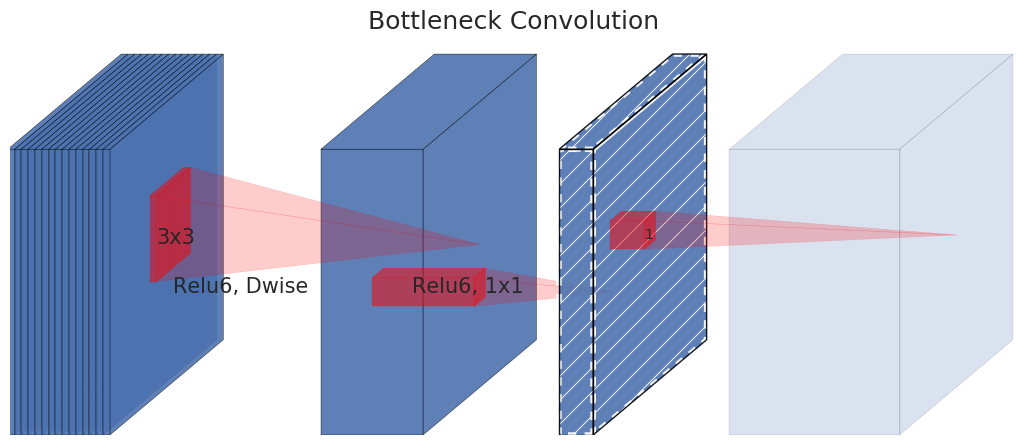
\includegraphics[width=0.6\textwidth]{content/images/bottleneck_block.png}}
\caption{Beispiel einer Linear Bottleneck Schicht. Die Breite jeder Schicht symbolisiert die Anzahl der Channel und auf den schraffierten Block wurde eine lineare Aktivierung angewendet. Der schwach sichtbare Block ist ein Block der nächsten Schicht. \cite{sandler_mobilenetv2_2019}}
\label{f2.3}
\end{figure}

Ein Beispiel für ein Linear Bottleneck aus dem Paper zu der Architektur MobileNetV2 \cite{sandler_mobilenetv2_2019} ist in Abbildung \ref{f2.2} dargestellt. Die Schicht besteht aus insgesamt 3 Convolutional Layern. Im ersten Schritt wird auf die Eingabe der Bottleneck Schicht eine nicht-lineare Aktivierungsfunktion (in dem Beispiel ReLU6) und anschließend eine Depthwise Convolution angewendet. Auf die Ausgabe der Depthwise Convolution wird erneut eine nicht-lineare Aktivierungsfunktion angewendet und es folgt eine Pointwise Convolution, welche die Eingabe auf eine komprimierte Repräsentation reduziert. Auf diese komprimierte Repräsentation wird zum Schluss eine lineare Aktivierungsfunktion angewendet und mittels Pointwise Convolution zu der Eingabe für die nächste Schicht transformiert.

\begin{figure}[htbp]
\centerline{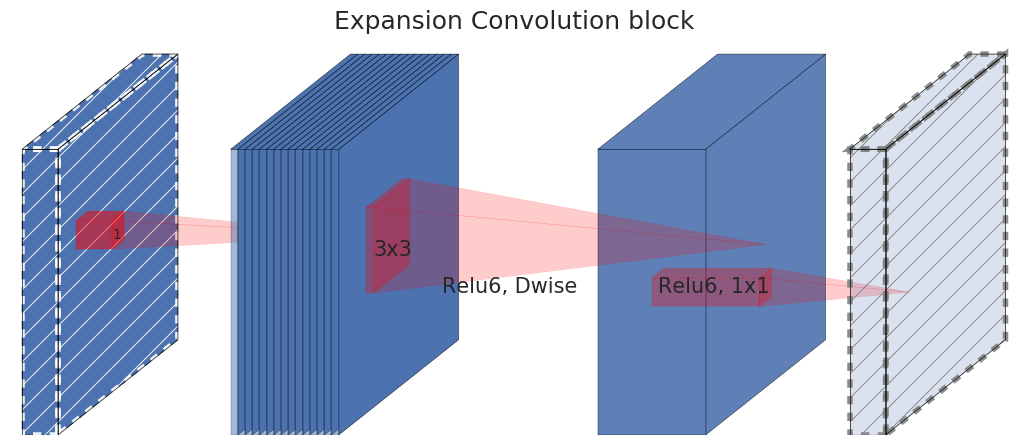
\includegraphics[width=0.6\textwidth]{content/images/expansion_block.png}}
\caption{Beispiel für einen Expansion Block. Die Breite jeder Schicht symbolisiert die Anzahl der Channel und auf die schraffierten Blöcke wurde eine lineare Aktivierung angewendet. Der schwach sichtbare Block ist ein Block der nächsten Schicht. \cite{sandler_mobilenetv2_2019}}
\label{f2.4}
\end{figure}

Werden mehrere von diesen Bottleneck Schichten hintereinandergeschaltet, ergibt sich eine Struktur, bei der immer wieder eine komprimierte Repräsentation in eine vergrößerte Repräsentation überführt wird und anschließend wieder in eine komprimierte Darstellung transformiert wird. Diese Blöcke werden auch Expansion Blöcke genannt und sind in Abbildung \ref{f2.4} dargestellt.

Das Paper zu MobileNetV2 beschreibt als Grund für die Anwendung der linearen Aktivierungsfunktion am Ende jeder Bottleneck Schicht, dass nicht-lineare Aktivierungsfunktionen zwar notwendig sind, um eine Nicht-Linearität des Modells zu erreichen, aber sie auch zu einer Zerstörung von Information führen. Außerdem haben Experimente gezeigt, dass die Anwendung einer linearen Aktivierungsfunktion in den Bottleneck Schichten zu einer Verbesserung des Netzwerkes führt \cite{sandler_mobilenetv2_2019}.


\subsection{Inverted Residuals}
\label{inverted_residuals}
Inverted Residuals \cite{sandler_mobilenetv2_2019} sind angelehnt an die Residual Blöcke der ResNet Architektur \cite{he_deep_2015}. Ein Residual Block in der ResNet Architektur nutzt ein Bottleneck Konstrukt, indem die Eingabe des Blocks mittels Convolutions komprimiert und anschließend wieder vergrößert wird. Zwischen der Eingabe und der Ausgabe des Residual Blocks befindet sich eine Abkürzung (Shortcut Connection), welche den Fluss der Gradienten im Trainingsprozess verbessert und es ermöglicht, tiefe Netze mit vielen Schichten besser zu trainieren \cite{he_deep_2015}.

Die Inverted Residual Blöcke verfolgen dieselbe Idee wie die Residual Blöcke beim ResNet, jedoch sind bei den Inverted Residual Blöcken die Schichten anders angeordnet. Ein Beispiel für ein Inverted Residual Block aus dem Paper zu der MobileNetV2 Architektur \cite{sandler_mobilenetv2_2019} ist in Abbildung \ref{f2.5} dargestellt. Der Unterschied bei den Inverted Residuals zu den Residual Blöcken ist, dass die Eingabe der Inverted Residual Schicht bereits die komprimierte Repräsentation ist, welche anschließend mittels einer Pointwise Convolution vergrößert wird. Darauf folgt eine Depthwise Convolution und erneut eine Pointwise Convolution, welche die Darstellung wieder komprimiert. Die Abkürzung befindet sich dabei zwischen dem Bottleneck am Eingang und der Bottleneck am Ausgang. Im Grunde handelt es sich um eine Expansion Schicht mit einer Abkürzung zwischen der Eingabe und der Ausgabe der Schicht.

\begin{figure}[htbp]
\centerline{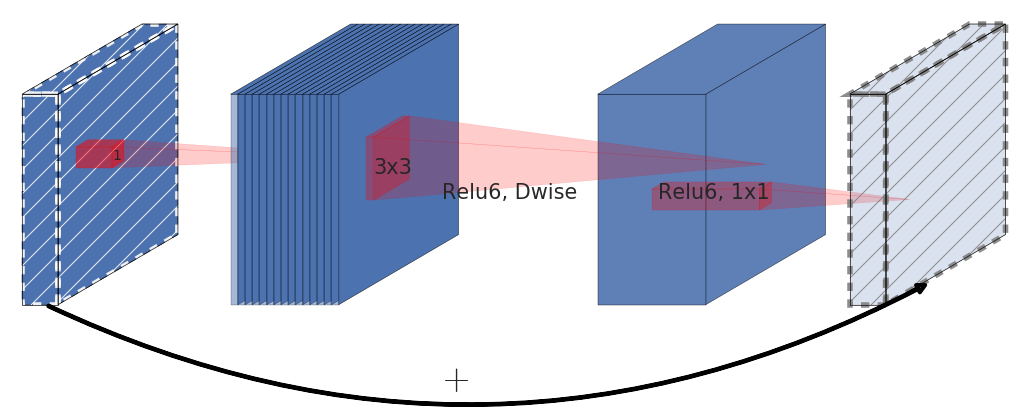
\includegraphics[width=0.6\textwidth]{content/images/inverted_residual.png}}
\caption{Inverted Residual Block. Die Breite jeder Schicht symbolisiert die Anzahl der Channel. \cite{sandler_mobilenetv2_2019}}
\label{f2.5}
\end{figure}

Bei der Abkürzung zwischen den Schichten handelt es sich lediglich um die Identitäts\-funktion. Das heißt, dass die Eingabe unverändert auf die Ausgabe addiert wird \cite{sandler_mobilenetv2_2019}.


\subsection{Squeeze-And-Excitation}
\label{squeeze_and_excitation}
Eine weitere Schicht sind die Squeeze-And-Excitation Schichten \cite{hu_squeeze-and-excitation_2019}. Der Grundgedanke hinter dieser Schicht ist es, die Beziehung zwischen den Kanälen (Channel) besser zu modellieren. Das Netzwerk soll die Möglichkeit haben wichtige Kanäle zu verstärken und weniger wichtige Kanäle abzuschwächen.

Diese Squeeze-And-Excitation Schicht, welche in Abbildung \ref{f2.6} dargestellt ist, kann nach beliebigen Transformationen $F_{tr}$ angewendet werden, die aus einer Eingabe $X$ der Größe $H' \times W' \times C'$ eine Feature Map $U$ der Größe $H \times W \times C$ generiert. Beispiele für mögliche Transformationen sind Convolutions oder Depthwise Convolutions.

\begin{figure}[htbp]
\centerline{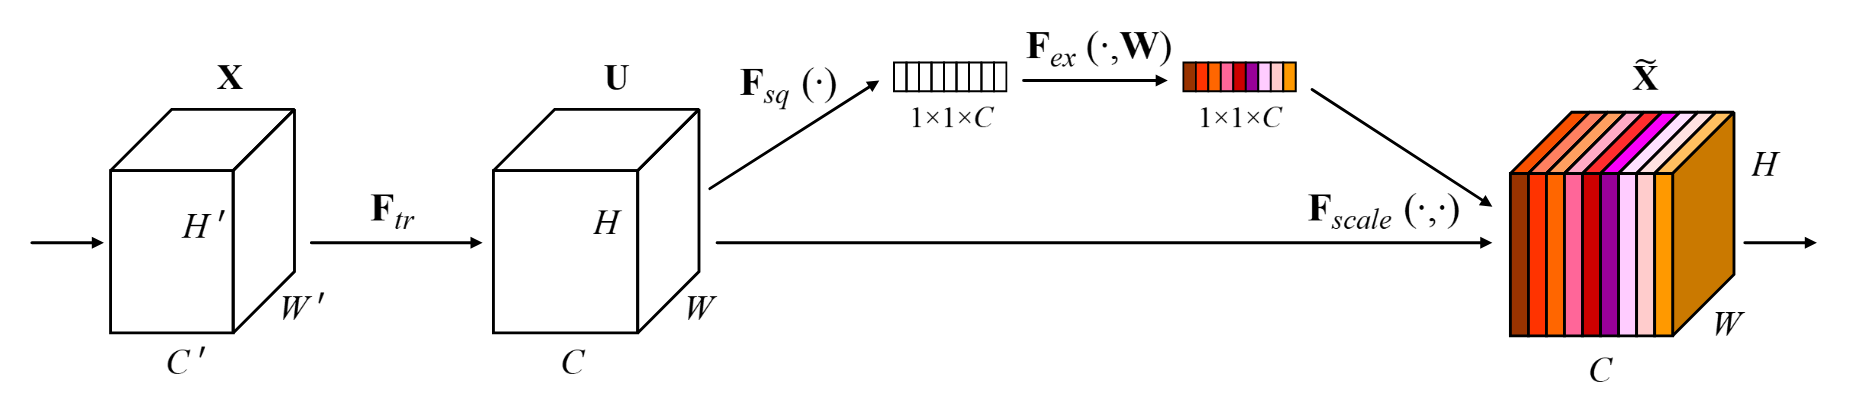
\includegraphics[width=0.9\textwidth]{content/images/squeeze_and_excitation.png}}
\caption{Ein Squeeze-And-Excitation Block. \cite{hu_squeeze-and-excitation_2019}}
\label{f2.6}
\end{figure}

Nach dieser Transformation wird auf die resultierende Feature Map die sogenannte Squeeze-Transformation angewendet, welche die Feature Map $U$ in eine Darstellung der Form $1 \times 1 \times C$ überführt. Dies kann zum Beispiel durch ein Global Average Pooling erreicht werden, welches für jeden Channel $u_c$ in $U = [u_1, u_2, \cdots, u_C]$ wie folgt berechnet wird \cite{hu_squeeze-and-excitation_2019}:

\begin{equation}
F_{sq}(u_c) = \frac{1}{H \cdot W} \sum_{i=1}^{H} \sum_{j=1}^{W} u_c[i, j]
\label{eq2.6}
\end{equation}

Darauf folgt die Excitation-Transformation, die auf das Ergebnis der Squeeze-Trans\-formation, analog zu den klassischen Feedforward-Netzen in Abschnitt \ref{FFNN}, mittels $F_{ex}$ eine Gewichtung $W$ und eine Aktivierung anwendet. Jedoch beinhaltet $F_{ex}$ noch ein Bottleneck, welcher in der Grafik \ref{f2.6} nicht ersichtlich ist. Das bedeutet $F_{ex}$ komprimiert zuerst mittels eines normalen Feedforward-Netzes die Darstellung der Größe $1 \times 1 \times C$ in einen Feature-Vektor der Größe $1 \times 1 \times \frac{C}{r}$ und wendet darauf eine Aktivierung an. Anschließend wird die komprimierte Darstellung wieder in die Darstellung der Größe $1 \times 1 \times C$ transformiert und erneut eine Aktivierung angewendet. $r$ ist dabei ein Parameter, der bestimmt, wie schmal der Bottleneck ist.

Die Ausgabe des Squeeze-And-Excitation Blockes wird nun mittels der Funktion $F_{scale}$ berechnet, welche lediglich die Channel aus der Feature Map $U$ mit den zugehörigen Channel aus dem Ergebnis von $F_{ex}$ multipliziert.



\section{Architekturen für Mobilgeräte}
\label{architekturen}
Nachdem die Grundlagen von künstlichen neuronalen Netzen und darauf aufbauende optimierte Schichten besprochen wurden, werden nun konkrete Architekturen für Convolutional Neural Networks vorgestellt, dessen Zielplattform mobile und eingebettete Systeme sind. Im Wesentlichen werden in diesem Abschnitt die verschiedenen MobileNet Varianten \cite{howard_mobilenets_2017, sandler_mobilenetv2_2019, howard_searching_2019} und die EfficientNet \cite{tan_efficientnet_2020} Architektur besprochen.


\subsection{MobileNet}
\label{mobilenet}
MobileNet \cite{howard_mobilenets_2017} ist eine Architektur aus dem Jahr 2017, welche von Entwicklern bei Google entwickelt wurde. Die Entwickler haben sich zum Ziel gesetzt, dem Trend, immer tiefere CNN Architekturen für eine gesteigerte Genauigkeit zu entwickeln, entgegenzuwirken, um die Verwendung von CNN Modellen auf mobilen und eingebetteten Systemen möglich zu machen. Dabei setzen sie den Hauptfokus bei der Entwicklung auf das Optimieren der Latenz, anstatt sich nur auf das Optimieren der Größe zu konzentrieren. Um dieses Ziel zu erreichen, haben die Entwickler die Architektur hauptsächlich aus Depthwise Separable Convolutions (siehe Abschnitt \ref{depthwise_separable_convolutions}) aufgebaut, welche die Berechnungskosten und die Größe des Netzwerkes stark reduzieren \cite{howard_mobilenets_2017}.

\begin{figure}[htbp]
\centerline{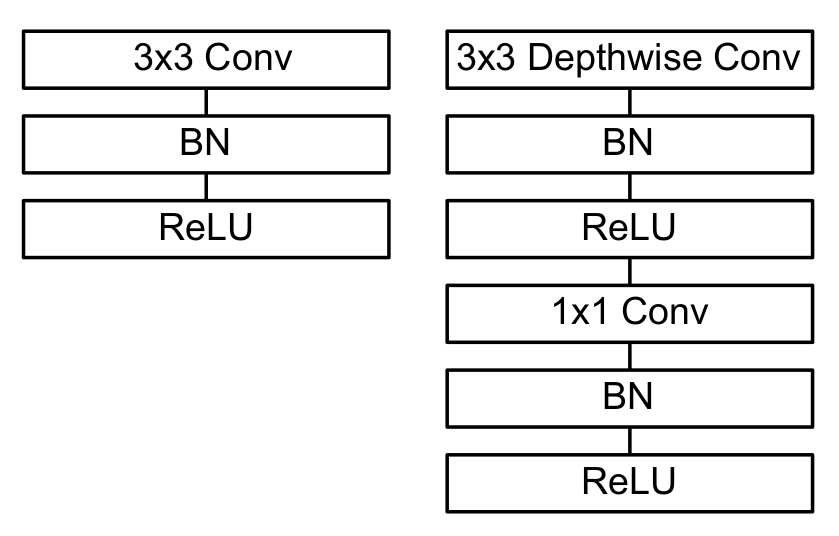
\includegraphics[width=0.3\textwidth]{content/images/mobilenet_blocks.png}}
\caption{Hauptbausteine des MobileNets. Links ist eine Standard-Convolution und rechts ist die Depthwise Separable Convolution. BN steht für Batch Normalisierung \cite{ioffe_batch_2015} und ReLU ist die ReLU Aktivierungsfunktion. \cite{howard_mobilenets_2017}}
\label{f2.7}
\end{figure}

Die MobileNet Architektur ist wie folgt aufgebaut. Sie beginnt mit der in Abbildung \ref{f2.7} dargestellten Standard-Convolution. Darauf folgen dann 13 Depthwise Separable Convolutions. Danach wird ein Average Pooling durchgeführt und das Ergebnis dieser Pooling-Operation wird mittels eines klassischen Feedforward-Netzes (Fully-Connected Layer) und einer Softmax Aktivierung als Klassifikator genutzt.

Um die Größe des MobileNets variieren zu können, gibt es noch einen Breitenmultiplikator (width multiplier) $\alpha$ und einen Auflösungsmultiplikator (resolution multiplier) $\rho$. Der Breitenmultiplikator skaliert gleichmäßig die Breite jeder Schicht, indem sich die Anzahl an Eingabe-Channel $M$ und Ausgabe-Channel $N$ in jeder Schicht zu $\alpha M$ und $\alpha N$ skalieren lassen.
Der Auflösungsmultiplikator $\rho$ wird in der Regel implizit gesetzt, indem die Auflösung des Eingabebildes verändert wird.


\subsection{MobileNetV2}
Im Jahr 2018 folgte auf die MobileNet Architektur die Nachfolgearchitektur MobileNetV2 \cite{sandler_mobilenetv2_2019}. Neben den Depthwise Separable Convolutions, welche bereits in der MobileNet Architektur Anwendung fanden, werden in dieser Architektur noch die Linear Bottlenecks (Abschnitt \ref{linear_bottlenecks}) und Inverted Residuals (Abschnitt \ref{inverted_residuals}) hinzugefügt.

Als Hauptbaustein nutzt die MobileNetV2 Architektur die Expansion Schicht mit residualer Verbindung wie sie in Abbildung \ref{f2.5} dargestellt ist. Diese Expansion Schichten werden in dem Paper auch Bottleneck Residual Block genannt. Mittels diesen Bottleneck Schichten wir nun die Architektur ähnlich zu MobileNet aufgebaut. 

Als erste Schicht kommt eine normale Standard-Convolution. Darauf folgen 17 Bottleneck Schichten. Von diesen Bottleneck Schichten besitzen alle Schichten, dessen Eingaben dieselbe Größe hat wie die Ausgaben, eine residuale Verbindung. Das ist für alle Bottleneck Schichten mit einer Schrittweite (Stride) von 1 der Fall. Bei den anderen Bottleneck Schichten handelt es sich um einfache Expansion Schichten. Nach diesen 17 Bottleneck Schichten folgt eine Pointwise Convolution und ein Average Pooling. Zur Klassifikation wird als letzte Schicht eine Pointwise Convolution verwendet. Als Aktivierungsfunktion wird in dieser Architektur ReLU6 eingesetzt.

Genau wie die MobileNet Architektur gibt es bei der MobileNetV2 Architektur den Breitenmultiplikator (width multiplier) $\alpha$ und den Auflösungsmultiplikator (resolution multiplier) $\rho$, die ermöglichen die Größe und Berechnungskosten der Architektur auf die Bedürfnisse anzupassen.


\subsection{MobileNetV3}
\label{mobilenetv3}
MobileNet und MobileNetV2 sind beides Architekturen, welche manuell von Menschen erdacht und konzipiert wurden. Die MobileNetV3 Architektur aus dem Jahr 2019 hingegen wurde mittels einer Platform-Aware Neural Architecture Search (Platform-Aware NAS) entwickelt \cite{howard_searching_2019}. Zusätzlich wurden noch einige manuelle Anpassungen vorgenommen. Von der MobileNetV3 Architektur gibt es eine kleine (Small) und eine große (Large) Variante.

Als Hauptbaustein der MobileNetV3 Architektur wird eine Linear Bottleneck Schicht mit Squeeze-And-Excitation und Inverted Residual verwendet wie in Abbildung \ref{f2.8} dargestellt. Als nichtlineare Aktivierungsfunktion wird dabei eine modifizierte Variante der Swish Aktivierungsfunktion \cite{howard_searching_2019} genutzt.

\begin{figure}[htbp]
\centerline{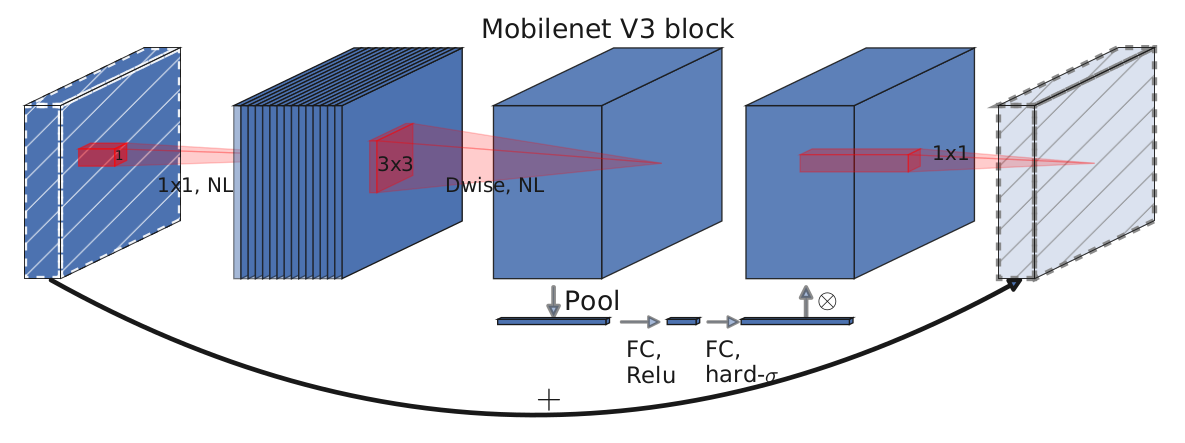
\includegraphics[width=0.7\textwidth]{content/images/mobilenetv3_block.png}}
\caption{Linear Bottleneck Schicht mit Squeeze-And-Excitation und Inverted Residual. \cite{howard_searching_2019}}
\label{f2.8}
\end{figure}

\subsubsection{MobileNetV3 Large}
Für die große Variante der MobileNetV3 Architektur wurde als Grundlage die durch Platform-Aware NAS gefundene Architektur MnasNet-A1 \cite{tan_mnasnet_2019} gewählt. Diese Architektur wurde mittels NetAdapt Algorithmus \cite{howard_searching_2019} weiter optimiert.
Anschließend wurden noch einige manuelle Anpassungen vorgenommen. 

Zu den manuellen Anpassungen gehören, dass teure Schichten überarbeitet wurden, indem die Anzahl der Filter der ersten Schicht verringert wurde und die letzten Schichten überarbeitet wurden, um eine geringere Latenz zu erreichen. Außerdem wurde ReLU6 als nichtlineare Aktivierungsfunktion durch eine modifizierte Variante der Swish Aktivierungsfunktion ersetzt, um die Genauigkeit der Architektur zu verbessern. Zusätzlich wurde die Skalierung des Squeeze-And-Excitation Bottlenecks angepasst.

Die MobileNetV3-Large Variante ist für mobile Plattformen mit einer größeren Anzahl an Ressourcen ausgelegt.


\subsubsection{MobileNetV3 Small}
Die kleine Variante des MobileNetV3 richtet sich an kleinere Plattformen mit einer geringen Menge an Ressourcen. Dazu baut diese Architektur nicht wie die große Variante auf der MnasNet-A1 Architektur auf, sondern wurde durch einen neuen Platform-Aware NAS Durchlauf gefunden. Platform-Aware Neural Architecture Search ist eine Technik, bei der eine optimale Architektur für eine bestimmte Plattform gesucht wird. Bei der MobileNetV3 Small Variante wurde bei dem NAS Algorithmus die Latenz und Genauigkeit der Architekturen auf real existierenden Mobilgeräten getestet und optimiert. Anschließend wurden dieselben Optimierungen wie auch bei der großen Variante angewendet.


\subsection{EfficientNet}
\label{efficientnet}
Eine weitere Architektur, welche mittels Neural Architecture Search entwickelt wurde, ist die EfficientNet Architektur aus dem Jahr 2019 \cite{tan_efficientnet_2020}. Die Entwickler haben sich bei dieser Architektur das Ziel gesetzt, eine Methode zu entwickeln, welche es erlaubt diese Architektur zu vergrößern und dabei eine bessere Genauigkeit zu erzielen, aber auch eine möglichst effiziente Architektur beizubehalten. Dazu haben sie die Compound Scaling Methode entwickelt.

Viele Architekturen lassen sich entweder nur in der Breite (Anzahl an Channel in den Schichten), in der Tiefe (Anzahl der Schichten) oder mittels der Auflösung des Eingabebildes skalieren. Beispielsweise lässt sich die MobileNet Architektur, wie in Abschnitt \ref{mobilenet} beschrieben, lediglich in der Breite und der Auflösung skalieren.
Die Idee hinter dem Compound Scaling ist es alle drei Arten der Skalierung zu verwenden, um eine Architektur gleichmäßig zu skalieren. Beim Compound Scaling wird ein Compound Koeffizient $\phi$ und Konstanten $\alpha$, $\beta$, $\gamma$ verwendet. Für die Konstanten muss gelten $\alpha \geq 1 \land \beta \geq 1 \land \gamma \geq 1$ und $\alpha \cdot \beta^2 \cdot \gamma^2 \approx 2$. Konkrete Werte für Konstanten $\alpha$, $\beta$, $\gamma$ wurden mittels einer Grid-Search ermittelt.
Anschließend wird die gegebene Basisarchitektur nach den folgenden Regeln skaliert \cite{tan_efficientnet_2020}:

\begin{itemize}
\item Tiefe: $d = \alpha^\phi$
\item Breite: $w = \beta^\phi$
\item Auflösung: $r = \gamma^\phi$
\end{itemize}

Um dieses Compound Scaling anwenden zu können, haben die Entwickler als Erstes mittels NAS Algorithmus eine Basisarchitektur entwickelt. Im Gegensatz zu MobileNetV3 wurde die Neural Architecture Search aber nicht für eine spezielle Hardware durchgeführt. Aus diesem Grund wurde anstelle nach Latenz und Genauigkeit nach Anzahl an Gleitkommazahlen-Operationen und Genauigkeit optimiert. Durch diese Suche ergab sich die Basisarchitektur EfficientNet-B0. Diese Architektur nutzt ähnlich wie die MobileNetV3 Architektur als Hauptbaustein die Linear Bottleneck Schichten mit Squeeze-And-Excitation und Inverted Residual. Als nichtlineare Aktivierungsfunktion wird die Swish Aktivierungsfunktion genutzt.

Auf Basis der EfficientNet-B0 Architektur wurden mittels der Compound Scaling Methode weitere Architekturen mit aufsteigender Anzahl an Parametern abgeleitet. Insgesamt gibt es 8 Architekturen (EfficientNet-B0 bis EfficientNet-B7), welche mit unterschiedlichen Werten für $\phi$ ermittelt wurden. Durch die Einschränkung $\alpha \cdot \beta^2 \cdot \gamma^2 \approx 2$ beim Compound Scaling gilt, dass wenn die Basisarchitektur mit einem $\phi$ vergrößert wird, vergrößert sich die Anzahl an Gleitkommazahlen-Operationen ungefähr um $2^\phi$. So können die Berechnungskosten auf die vorhandenen Ressourcen eingestellt werden.

Auf den normalen EfficientNet Architekturen aufbauend wurden im Jahr 2020 zusätzlich die EfficientNet-lite \cite{liu_higher_2020} Architekturen veröffentlicht. Die Idee hinter den EfficientNet-lite Architekturen ist auf dem EfficientNet basierende Architekturen bereitzustellen, die eine höhere Kompatibilität mit verschiedener Hardware aufweisen, weniger Parameter besitzen und sich besser quantisieren lassen. Dazu wurden zum einen die Squeeze-And-Excitation Module entfernt, da sie teilweise nicht gut unterstützt werden und zum anderen wurde die Swish Aktivierungsfunktion durch ReLU6 ausgetauscht, um eine bessere Quantisierbarkeit zu ermöglichen. Außerdem wurden einige Parameter beim Compound Scaling ausgeschlossen, da dadurch die Anzahl an Berechnungen verringert wird. Es gibt insgesamt fünf EfficientNet-lite Varianten (EfficientNet-lite0 bis EfficientNet-lite4), welche aufsteigend viele Parameter besitzen.



\section{Quantisierung}
\label{quantisierung}
Im vorherigen Abschnitt wurden Architekturen vorgestellt, welche versprechen eine gute Performance auf mobiler und eingebetteter Hardware zu besitzen. Zusätzlich zum Aufbau der Architektur lässt sich mittels Techniken wie Quantisierung die Effizienz in Bezug auf Inferenzgeschwindigkeit und Speicherbedarf weiter optimieren.

Bei der Quantisierung geht es darum, die Gewichte und Aktivierungen eines Netzwerkes in eine Darstellung zu überführen, welche weniger Bits als die ursprüngliche Darstellung benötigen. Ein Beispiel für eine Quantisierung ist, das Überführen eines Netzwerkes, welches 32 Bit Fließkommazahlen für die Gewichte/Aktivierungen verwendet, in ein Netzwerk, welches lediglich 8 Bit Integer verwendet. Dabei können die Gewichte und Aktivierungen in unterschiedliche Bitlängen quantisiert werden \cite{jacob_quantization_2017}.

Quantisierung hat dadurch den Vorteil, dass durch die verkleinerte Repräsentation der Gewichte und Aktivierungen der Gesamtspeicherbedarf eines Netzwerkes sinkt. Außerdem wird durch die Quantisierung in Integer die Geschwindigkeit des Netzwerkes auf Hardware, welche lediglich Integer-Operationen unterstützt, erhöht \cite{jacob_quantization_2017}.

Um ein gegebenes Netzwerk zu quantisieren, wurden im Laufe der Zeit verschiedene Ansätze entwickelt \cite{guo_survey_2018}. In dieser Arbeit wird im Wesentlichen das Quantisierungsschema der TensorFlow Bibliothek vorgestellt \cite{jacob_quantization_2017}. Dieses Quantisierungsschema bietet zwei Möglichkeiten eine Quantisierung vorzunehmen. Zum einen kann ein bereits vollständig trainiertes und bisher noch nicht quantisiertes Netz nachträglich quantisiert werden. Dies wird als Post-Training Quantization bezeichnet. Eine andere Möglichkeit, die als Quantization-Aware Training bezeichnet wird, ist das Trainieren eines Full-Precision Modells so als wäre es quantisiert. Im Folgenden werden diese beiden Möglichkeiten genauer betrachtet.


\subsection{Post-Training Quantization}
\label{post-training-quantization}
Bei der Post-Training Quantization wird als Grundlage ein bereits trainiertes neuronales Netz verwendet. Von diesem Netz werden dann die Gewichte und/oder Aktivierungen nachträglich quantisiert. Um dies zu erreichen wird ein reeller Wert $r$ (z.B. ein Gewicht des Netzes als 32 Bit Fließkommazahl) wie folgt durch einen quantisierten Wert $q$ (z.B. 8 Bit Integer) dargestellt \cite{jacob_quantization_2017}:

\begin{equation}
r = S (q - Z)
\label{eq2.7}
\end{equation}

In dieser Formel sind $S$ und $Z$ Konstanten. Dabei steht $S$ für "`scale"' und entspricht demselben Typ wie der nicht quantisierte Wert $r$. Die Konstante $Z$ steht für "`zero-point"' und hat denselben Typ wie der quantisierte Wert $q$. $Z$ entspricht dem quantisierten Wert für den die reelle Zahl 0 ($r = 0$). Diese beiden Konstanten werden auch als Quantisierungsparameter bezeichnet und für jede Gewichtsmatrix neu bestimmt.

Mit dieser Formel ist es möglich, sämtliche Parameter des Modells zu quantisieren, indem man jeden zu quantisierenden Parameter $r$ als einen Wert $q$ mit den Konstanten $S$ und $Z$ darstellt. Aufbauend auf diesem Quantisierungsschema lassen sich effiziente Operationen wie Matrizenmultiplikationen definieren, welche nur auf den quantisierten Werten (Integer) arbeiten \cite{jacob_quantization_2017}.

Wird mittels dieses Schemas ein bereits trainiertes Full-Precision Modell nachträglich quantisiert, funktioniert dies bei großen Modellen häufig gut. Bei kleineren Modellen kann dies zu größeren Einbußen in der Genauigkeit des Modells führen \cite{jacob_quantization_2017}. Gründe dafür können zum einen sein, dass die Gewichte zwischen den einzelnen Ausgabekanälen einer Schicht zu weit voneinander entfernt sind. Zum anderen kann es aber auch daran liegen, dass es Ausreißer in den Gewichten gibt, welche die Präzision der anderen Gewichte in quantisierter Form verschlechtern \cite{jacob_quantization_2017}.


\subsection{Quantization-Aware Training}
\label{quantization_aware_training}
Um diesem Problem entgegen zu wirken gibt es den Ansatz des Quantization-Aware Training. Bei diesem Ansatz wird ein Full-Precision Modell trainiert und dabei die Auswirkungen von Quantisierung lediglich simuliert.

Dazu wird beim Training im Foreward-Pass die Eingabe, Gewichte und Aktivierungsfunktionen so berechnet als wäre das Model quantisiert. Anschließend wird der Fehler berechnet, den das Netzwerk gemacht hat und beim Backward-Pass wie bei einem nicht quantisierten Full-Precision Modell die Gewichte angepasst. Die Gewichte werden jedoch in dem Typ des nicht quantisierten Modells gespeichert und können somit beim Backward-Pass sehr feingranular angepasst werden.

Nach diesem Training ergibt sich ein trainiertes Full-Precision Modell, welches so trainiert wurde als wäre es quantisiert. Dieses Modell kann anschließend mittels Post-Training Quantization in eine quantisierte Repräsentation überführt werden.



\section{Pruning}
\label{pruning}
Neben der Quantisierung gibt es als weitere Optimierungstechnik das sogenannte Pruning (Beschneiden). Beim Pruning wird ein Netzwerk optimiert, indem Verbindungen unterbrochen werden, welche keinen signifikanten Beitrag zur Ausgabe des Netzwerkes leisten. Mit Verbindungen unterbrechen ist in dem Zusammenhang das auf 0 setzen von Gewichten gemeint. Durch ein angemessenes Pruning kann die Größe eines Modells drastisch reduziert werden mit meist geringen Einbußen in der Genauigkeit \cite{zhu_prune_2017}.

Um ein gegebenes Netzwerk zu prunen gibt es verschiedene Ansätze \cite{gale_state_2019, mishra_survey_2020}. In dieser Arbeit wird der Ansatz des Magnitude Pruning \cite{zhu_prune_2017} genauer betrachtet, da es sich beim Magnitude Pruning um einen einfachen und effektiven Ansatz handelt, welcher trotz der Einfachheit gute Ergebnisse erzielt.

\subsection{Magnitude Pruning}
\label{magnitude_pruning}
Beim Magnitude Pruning wird bei einem gegebenen Netzwerk für jede Gewichtsmatrix eine binäre Maske derselben Größe erzeugt. Die einzelnen Einträge in dieser binären Maske geben an, welche der Gewichte beim Training berücksichtigt werden und welche nicht. Anschließend werden die einzelnen Gewichte nach ihrem Wert sortiert und in der Maske die kleinsten Gewichte auf 0 gesetzt bis ein Prozentsatz $s$ (Sparsity) erreicht wurde, welcher den Anteil der auf 0 gesetzten Gewichte in dem Netzwerk angibt \cite{zhu_prune_2017}.

In der Magnitude Pruning Methode aus dem Jahr 2017 \cite{zhu_prune_2017}, welche hier beschrieben wird, besteht der Pruningprozess aus einer mehrfachen wechselweisen Abfolge von Pruning und Training. Dazu wurde ein Algorithmus zum schrittweisen Prunen von neuronalen Netzen entwickelt. Dieser Algorithmus beginnt bei einer Sparsity von $s_i$ Prozent und erhöht $n$ Mal alle $\Delta t$ Schritte den Anteil der auf 0 gesetzten Gewichte bis zu einem gewünschten Prozentsatz $s_f$. Der Startpunkt, ab wann der Pruningprozess im Verlauf des Trainingsprozesses beginnt, kann mit dem Parameter $t_0$ festgelegt werden. Der Anteil $s_t$ der auf 0 gesetzten Gewichte im Pruningschritt $t$ wird nach folgender Formel berechnet \cite{zhu_prune_2017}:

\begin{eqnarray}
s_t = s_f + \left( s_i - s_f \right) \left( 1 - \frac{t - t_0}{n \Delta t} \right)^3
& \textrm{für} 
& t \in \{ t_0, t_0 + \Delta t, \cdots, t_0 + n \Delta t \}
\label{eq2.8}
\end{eqnarray}

Die Idee hinter diesem schrittweisen Pruning ist, dass nach jedem Pruningschritt das Netzwerk durch das anschließende Training die Möglichkeit bekommt sich an diesen Eingriff anzupassen und mögliche Verluste durch das Pruning auszugleichen bevor erneut ein Pruningschritt folgt. In Abbildung \ref{f2.9} ist ein Beispiel für einen schrittweisen Pruningvorgang nach der Formel \ref{eq2.8} dargestellt, in der zu erkennen ist, dass am Anfang des Pruningprozesses die Anzahl der Gewichte, die auf 0 gesetzt werden, größer ist und im Verlauf des Prozesses das Netz immer weniger stark gepruned wird, bis die gewünschte Sparsity $s$ erreicht wurde. Der Grund dafür ist, dass angenommen wird, dass am Anfang des Pruningvorgangs viele unwichtige Gewichte im Netzwerk existieren und mit zunehmender prozentualer Sparsity weniger unwichtige Gewichte im Netz vorhanden sind \cite{zhu_prune_2017}.

\begin{figure}[htbp]
\centerline{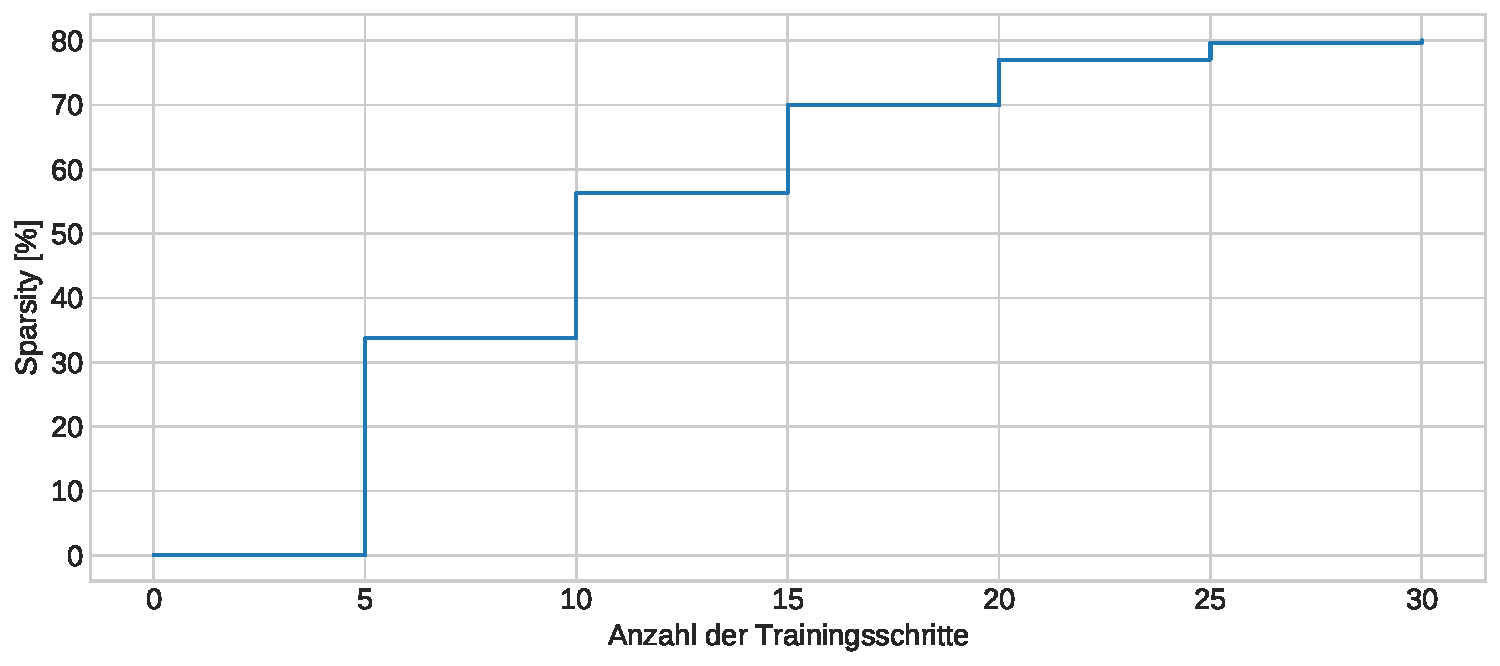
\includegraphics[width=0.9\textwidth]{content/images/magnitude_pruning_schedule.pdf}}
\caption{Ein Beispiel für einen Pruningprozess nach der Formel \ref{eq2.8} mit den Parametern $s_i = 0$, $s_f = 80$, $t_0 = 0$, $\Delta t = 5$ und $n = 6$.}
\label{f2.9}
\end{figure}
